% This file was created with tikzplotlib v0.10.1.
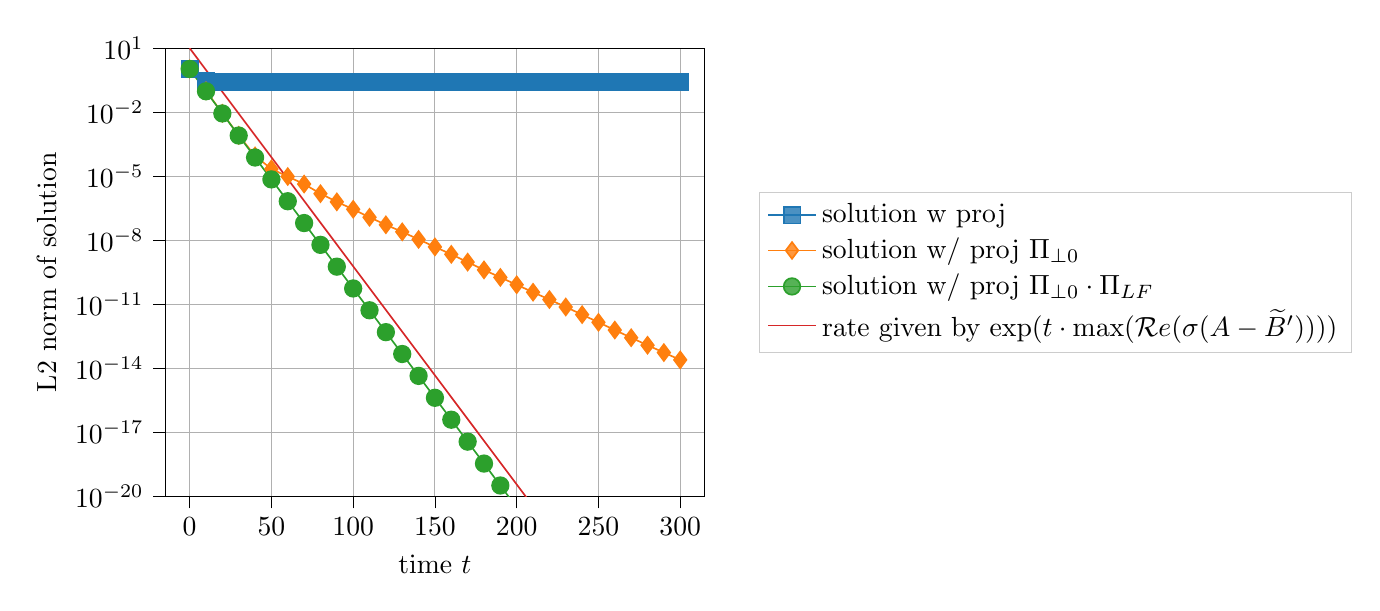
\begin{tikzpicture}

\definecolor{crimson2143940}{RGB}{214,39,40}
\definecolor{darkgray176}{RGB}{176,176,176}
\definecolor{darkorange25512714}{RGB}{255,127,14}
\definecolor{forestgreen4416044}{RGB}{44,160,44}
\definecolor{lightgray204}{RGB}{204,204,204}
\definecolor{steelblue31119180}{RGB}{31,119,180}

\begin{axis}[
legend cell align={left},
legend style={
  fill opacity=0.8,
  draw opacity=1,
  text opacity=1,
  at={(1.1,0.5)},
  anchor=west,
  draw=lightgray204
},
log basis y={10},
tick align=outside,
tick pos=left,
x grid style={darkgray176},
xlabel={time $t$},
xmajorgrids,
xmin=-15, xmax=315,
xtick style={color=black},
y grid style={darkgray176},
ylabel={L2 norm of solution},
ymajorgrids,
ymin=1e-20, ymax=10,
ymode=log,
ytick style={color=black},
ytick={1e-23,1e-20,1e-17,1e-14,1e-11,1e-08,1e-05,0.01,10,10000},
yticklabels={
  $\mathdefault{10^{-23}}$,
  $\mathdefault{10^{-20}}$,
  $\mathdefault{10^{-17}}$,
  $\mathdefault{10^{-14}}$,
  $\mathdefault{10^{-11}}$,
  $\mathdefault{10^{-8}}$,
  $\mathdefault{10^{-5}}$,
  $\mathdefault{10^{-2}}$,
  $\mathdefault{10^{1}}$,
  $\mathdefault{10^{4}}$
}
]
\addplot [semithick, steelblue31119180, mark=square*, mark size=3, mark options={solid}]
table {%
0 1.05962445391129
10 0.271579530169706
20 0.252064140997236
30 0.251707297796384
40 0.251681161835677
50 0.25167866869459
60 0.25167850379256
70 0.251678491832658
80 0.251678491442509
90 0.251678491464909
100 0.251678491476725
110 0.251678491475561
120 0.251678491474631
130 0.251678491473797
140 0.251678491473344
150 0.251678491473303
160 0.251678491473285
170 0.25167849147326
180 0.251678491473251
190 0.251678491473249
200 0.251678491473248
210 0.251678491473248
220 0.251678491473248
230 0.251678491473248
240 0.251678491473248
250 0.251678491473248
260 0.251678491473248
270 0.251678491473248
280 0.251678491473248
290 0.251678491473248
300 0.251678491473248
};
\addlegendentry{solution w\ proj}
\addplot [semithick, darkorange25512714, mark=diamond*, mark size=3, mark options={solid}]
table {%
0 1.05962445391129
10 0.100799928570626
20 0.00888996419928036
30 0.000823334716387433
40 9.00436389580916e-05
50 2.19784619826149e-05
60 9.69078544496262e-06
70 4.31770203484635e-06
80 1.531327399808e-06
90 6.32934081785688e-07
100 2.83416836897527e-07
110 1.19519078783243e-07
120 5.32660398381808e-08
130 2.4820910330745e-08
140 1.10043841758883e-08
150 4.89968484911718e-09
160 2.19719979573471e-09
170 9.50061789303546e-10
180 4.09650155918546e-10
190 1.82923954182744e-10
200 8.24609697174385e-11
210 3.70392255264194e-11
220 1.67583704238651e-11
230 7.50601577229445e-12
240 3.29750256768072e-12
250 1.43709077179439e-12
260 6.25434411151971e-13
270 2.73570789026002e-13
280 1.21768770730232e-13
290 5.50922252588842e-14
300 2.50059742374348e-14
};
\addlegendentry{solution w/ proj $\Pi_{\perp 0}$}
\addplot [semithick, forestgreen4416044, mark=*, mark size=3, mark options={solid}]
table {%
0 1.05962445391129
10 0.0955215283164192
20 0.00872709845052959
30 0.000807483575033667
40 7.55224354166436e-05
50 7.12194362312964e-06
60 6.75381493260096e-07
70 6.42523358471142e-08
80 6.12035423254634e-09
90 5.82890438104887e-10
100 5.54487864022824e-11
110 5.26535874460931e-12
120 4.98954910374828e-13
130 4.71803473666431e-14
140 4.45222983557405e-15
150 4.19397393935627e-16
160 3.94523533294454e-17
170 3.70788972324616e-18
180 3.48355228799717e-19
190 3.27345083944987e-20
200 3.07833599884726e-21
210 2.89843007022948e-22
220 2.73341889503217e-23
230 2.58248981685172e-24
240 2.44441425223163e-25
250 2.31766668312186e-26
260 2.20056553025092e-27
270 2.09141772320652e-28
280 1.98864915399293e-29
290 1.89090724718026e-30
300 1.79712797747339e-31
};
\addlegendentry{solution w/ proj $\Pi_{\perp 0}\cdot\Pi_{LF}$}
\addplot [semithick, crimson2143940]
table {%
0 10
10 0.951111830888997
20 0.090461371485702
30 0.00860388806584957
40 0.000818325973107418
50 7.78319514546217e-05
60 7.40268898496687e-06
70 7.04078507399366e-07
80 6.69657398262203e-08
90 6.36919074129526e-09
100 6.05781266723458e-10
110 5.76165729711604e-11
120 5.47998042081499e-12
130 5.2120742112772e-13
140 4.95726544581719e-14
150 4.71491381437395e-15
160 4.48441031047303e-16
170 4.2651757008515e-17
180 4.05665906990013e-18
190 3.85833643526517e-19
200 3.66970943113078e-20
210 3.49030405587341e-21
220 3.31966948094105e-22
230 3.15737691796417e-23
240 3.00301854125156e-24
250 2.85620646296337e-25
260 2.71657175838608e-26
270 2.58376353885993e-27
280 2.45744807002931e-28
290 2.3373079332002e-29
300 2.22304122769743e-30
};
\addlegendentry{rate given by $\exp(t\cdot\max(\mathcal{R}e(\sigma(A-\widetilde{B}'))))$}
\end{axis}

\end{tikzpicture}
